%%%%%%%% Klassen-Optionen
\documentclass[12pt,a4paper]{scrartcl}

%%%%%%%% PAKETE: unverzichtbare Pakete mit Einstellungen
\usepackage[left=2.5cm, right=2cm, top=3cm, bottom=3cm, a4paper]{geometry} %Seitenrände
\usepackage[utf8x]{inputenc} % utf8-Kodierung und direkte Eingabe von Sonderzeichen
\usepackage{fixltx2e} % Verbessert einige Kernkompetenzen von LaTeX2e

%%%%%%%% PAKETE: AMS-Pakete
\usepackage{amsmath} % Mathe-Erweiterung
\usepackage{amsfonts} % Schrift-Erweiterung
\usepackage{amssymb} % Sonderzeichen-Erweiterung

%%%%%%%% PAKETE: Sonstiges
\usepackage[colorlinks, citecolor=black, filecolor=black, linkcolor=black, urlcolor=black]{hyperref} % Links
\usepackage{wrapfig} % ausgeklügekte Floatumgebung
\usepackage{float} % normale Floatumgebung
\restylefloat{figure} % ermöglicht die Verwendung von "H" (ist noch stärker als "h!")
\usepackage[small,it,singlelinecheck=false]{caption} % Bildunterschriften formatieren
\usepackage{multirow} % ermöglich Verbinden von Tabellenzeilen
\usepackage{multicol} % ermöglicht Spalten
\usepackage{fancyhdr} % ermöglicht Kopf- und Fußzeilen
\usepackage{graphicx} % Einbinden von Bildern möglich
\usepackage{units} % Einheiten
\usepackage{subcaption}

%%%%%%%% DEFINITIONEN: Titelseite
\author{April Cooper, Patrick Kreissl und Sebastian Weber}
\title{Worksheet 1: Quantum mechanical approaches:
Hückel approximation and DFT methods}
\publishers{University of Stuttgart}
\date{\today}

%%%%%%%% ANPASSUNGEN: Kopf-und Fußzeile
\fancypagestyle{plain}{} % redefine the plain pagestyle to match the fancy layout
\pagestyle{fancy} % aktiviere eigenen Seitenstil
\fancyhf{} % alle Kopf- und Fußzeilen bereinigen
\fancyhead[L]{Worksheet 1: Quantum mechanical approaches}
\fancyhead[R]{\today}
\renewcommand{\headrulewidth}{0.6pt} % obere Trennlinie
\fancyfoot[L]{April Cooper, Patrick Kreissl und Sebastian Weber}
\fancyfoot[R]{Page \thepage}
\renewcommand{\footrulewidth}{0.6pt} % untere Trennlinie

%%%%%%%% ANPASSUNGEN: Absätze
\setlength{\parindent}{0em} % keine Absatzeinzüge
\setlength{\parskip}{0em} % Absatz-Abstand

%%%%%%%% ANPASSUNGEN: Abbildungsverzeichnis
\usepackage{tocloft} % Zum Anpassen der Verzeichnisse
%\renewcommand{\cftfigpresnum}{Abb. }
%\renewcommand{\cfttabpresnum}{Tab. }
\renewcommand{\cftfigaftersnum}{:}
\renewcommand{\cfttabaftersnum}{:}
\setlength{\cftfignumwidth}{2cm}
\setlength{\cfttabnumwidth}{2cm}
\setlength{\cftfigindent}{0cm}
\setlength{\cfttabindent}{0cm}

%%%%%%%% SONSTIGES
\usepackage{pdfpages}
\usepackage{pgf}
%\usepackage{subfigure}
\usepackage{graphicx}
\usepackage{caption}
\usepackage{subcaption}

% NÜTZLICH: http://truben.no/latex/table/

% Anfang des eigentlichen Dokuments
\begin{document}

\maketitle
\tableofcontents
\newpage

% =============== Section ============
\section{Computational Task: DFT calculations with Siesta}

\subsection{Geometry optimization of adenine}

\begin{tabular}{|c|c|c|c|c|c|c|c|c|c|}
\hline 
Distance & Here & Ref [20] & Ref [7] & Exp & Angle & Here & Ref [20] & Ref [7] & Exp \\ 
\hline 
C2-N3 & • & • & • & • & • & • & • & • & • \\ 
\hline 
N1-C2 & • & • & • & • & • & • & • & • & • \\ 
\hline 
C6-N1 & • & • & • & • & • & • & • & • & • \\ 
\hline 
C5-C6 & • & • & • & • & • & • & • & • & • \\ 
\hline 
C4-C5 & • & • & • & • & • & • & • & • & • \\ 
\hline 
N3-C4 & • & • & • & • & • & • & • & • & • \\ 
\hline 
\end{tabular} 

\newpage

\subsection{Theoretical Prediction of Watson-Crick Hydrogen-bond length in
adenine-thymine base pair}

\begin{figure}[H]
        \centering
        \begin{subfigure}[b]{0.49\textwidth}
                \centering
                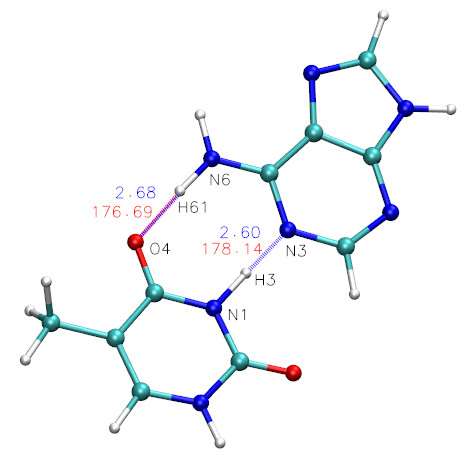
\includegraphics[width=\textwidth]{lda.jpg}
                \caption{LDA}
                \label{fig:gull}
        \end{subfigure}
        \begin{subfigure}[b]{0.49\textwidth}
                \centering
                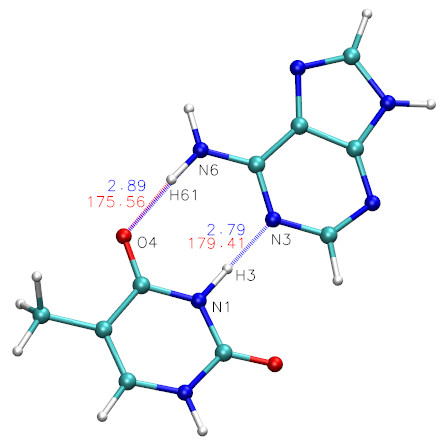
\includegraphics[width=\textwidth]{gga.jpg}
                \caption{GGA}
                \label{fig:tiger}
        \end{subfigure}
        \caption{Results for two flavours of XC functional. Blue numbers show bond lengths and red ones show bond angles.}\label{fig:ade-thy}
\end{figure}

\begin{table}[H]
\begin{tabular}{l||l|l|l}
Angle in \r{A} & LDA & GGA & Literature \footnotemark[1]\\ 
\hline \hline 
O4-H61-N6 & 176.7 & 175.6 & 175.8\\ 
\hline 
N1-H3-N3 & 178.1 & 179.4 & 178.1\\ 
\end{tabular}
\caption{Bond angles}\label{tab:angles}
\end{table}

\begin{table}[H]
\begin{tabular}{l||l|l|l|l}
Distance in \r{A} & LDA & GGA & Experiment 1 \footnotemark[1] & Experiment 2 \footnotemark[1] \\ 
\hline \hline 
O4-N6 & 2.68 & 2.89 & 2.95 & 2.93 \\ 
\hline 
N1-N3 & 2.60 & 2.79 & 2.82 & 2.85 \\ 
\end{tabular}
\caption{Bond lengths}\label{tab:lengths}
\end{table}

\footnotetext[1]{source: Attachment1b.pdf}

TODO: Write some text. Write down number of steps.

\end{document}


% =============== Comments ============
\begin{comment}
\verb{x_init {}}

\begin{figure}[H]
	\resizebox{1\textwidth}{!{\input{../plots/NAME.pgf}}
	\caption{CAPTION}\label{fig:NAME}
\end{figure}
\end{comment}
